\documentclass[aspectratio=169]{beamer}
\useoutertheme[progressbar=frametitle]{metropolis}
\useinnertheme{metropolis}
\definecolor{nabgray}{rgb}{0.6,0.59,0.61}
\usecolortheme[named=nabgray]{structure}
\usepackage{tikz}
\usepackage[utf8]{inputenc}
\usepackage[spanish]{babel}
\usepackage{fontspec}
\setmonofont{JetBrains Mono}
\setmainfont{Roboto}
\setsansfont{Roboto}

\usepackage{smartdiagram}
\usepackage{qtree}
\usepackage{verbatim}
\usepackage{svg}
\usepackage{graphicx}
\usepackage{color}
\definecolor{lightgray}{rgb}{0.95, 0.95, 0.95}
\definecolor{darkgray}{rgb}{0.4, 0.4, 0.4}
\definecolor{ocherCode}{rgb}{1, 0.5, 0} % #FF7F00 -> rgb(239, 169, 0)
\definecolor{blueCode}{rgb}{0, 0, 0.93} % #0000EE -> rgb(0, 0, 238)
\definecolor{greenCode}{rgb}{0, 0.6, 0} % #009900 -> rgb(0, 153, 0) 

\usepackage{upquote}
\usepackage{listings}
\lstset{language=java,
    otherkeywords={var,record},
	% Basic design
	backgroundcolor=\color{lightgray},
	basicstyle={\small\ttfamily},   
	frame=l,
	keywordstyle=\footnotesize\color{blue},
	escapeinside={<@}{@>},
	breaklines=true,
	% Line numbers
	xleftmargin={0.75cm},
	numbers=left,
	stepnumber=1,
	firstnumber=1,
	numberfirstline=true
	% Code design
	identifierstyle=\color{black},
	keywordstyle=\color{ocherCode}\bfseries,
	ndkeywordstyle=\color{greenCode}\bfseries,
	stringstyle=\color{ocherCode}\ttfamily,
	commentstyle=\color{darkgray}\ttfamily,
	tabsize=2,
	showtabs=true,
	showspaces=false,
	showstringspaces=false,
	extendedchars=true,
	breaklines=true
}

\lstdefinelanguage{bash}{
    basicstyle=\ttfamily,
    showstringspaces=false,
    commentstyle=\color{red},
    keywordstyle=\color{blue},
    numbers=right,
    xleftmargin={0.25cm}
}

\usebackgroundtemplate
{
	
\includegraphics[width=\paperwidth]{Images/fondo}%
}


\title{Cursos 2020}
\author{Víctor Orozco - @tuxtor}
\institute{Academik}
\date{\today}

\begin{document}

{
    \usebackgroundtemplate{
\includegraphics[width=\paperwidth]{Images/separador}}
    \setbeamercolor{normal text}{fg=white}
    \setbeamercolor{frametitle}{fg=red}
    \usebeamercolor[fg]{normal text}
    \frame{\titlepage}
}


{
	\usebackgroundtemplate{
\includegraphics[width=\paperwidth]{Images/separador}}
	\setbeamercolor{normal text}{fg=white}
	\setbeamercolor{frametitle}{fg=red}
	\usebeamercolor[fg]{normal text}
	\section{Antecedentes}
}

\begin{frame}[fragile]{Antecedentes}
	\begin{itemize}
		\item Nabenik S.A.
		\item Proveedores de consultoria de TELUS International
		\item Bootcamps de programación prácticos por licitación
		\item Subsidiados
	\end{itemize}	
\end{frame}

\begin{frame}[fragile]{Antecedentes}
	\begin{figure}
		\centering
		
\includegraphics[width=0.5\linewidth]{Images/awards}
	\end{figure}
\end{frame}

\begin{frame}[fragile]{Antecedentes}
\begin{figure}
	\centering
	
\includegraphics[width=0.9\linewidth]{Images/backendviejo}
\end{figure}
\end{frame}

\begin{frame}[fragile]{Antecedentes}
	Resultados
	\begin{itemize}
		\item 500 alumnos durante el primer año
		\item 3 personas que no sabian nada de programación ya trabajan en el medio
		\item Segmento calidad
	\end{itemize}	
\end{frame}


{
	\usebackgroundtemplate{
\includegraphics[width=\paperwidth]{Images/separador}}
	\setbeamercolor{normal text}{fg=white}
	\setbeamercolor{frametitle}{fg=red}
	\usebeamercolor[fg]{normal text}
	\section{Mercado y propuesta}
}


\begin{frame}[fragile]{Mercado laboral Ing. en Sistemas}
	\begin{figure}
		\centering
		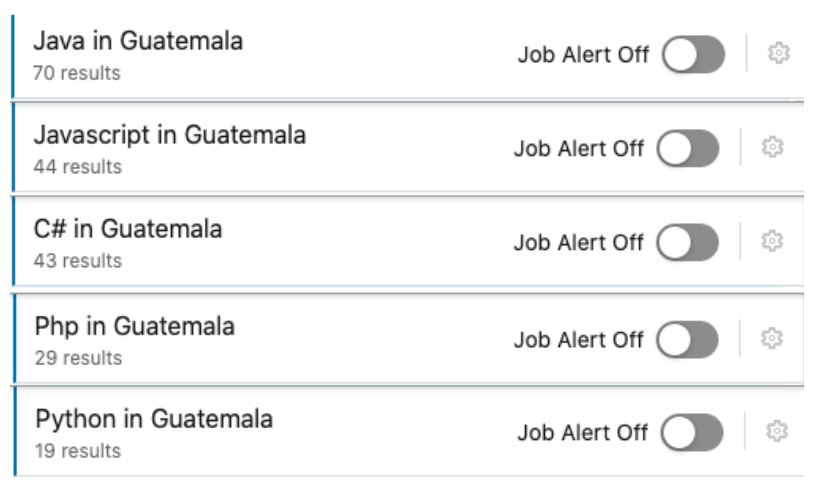
\includegraphics[width=0.9\linewidth]{Images/trabajos}
	\end{figure}

\end{frame}

\begin{frame}[fragile]{Diplomado 1}
	\begin{figure}
		\centering
		
\includegraphics[width=\linewidth]{Images/frontend}
	\end{figure}
	
\end{frame}

\begin{frame}[fragile]{Diplomado 2}
	\begin{figure}
		\centering
		
\includegraphics[width=\linewidth]{Images/backend}
	\end{figure}
	
\end{frame}
\begin{frame}[fragile]{Propuesta de valor}
	\begin{itemize}
		\item Cursos de 40 horas
		\item Codificación en tiempo real
		\item Conocimiento práctico para obtener trabajo
		\item Complementa la Universidad en lugar de competir con ella
	\end{itemize}	
\end{frame}

\begin{frame}[fragile]{Propuesta de valor}
	\begin{itemize}
		\item Programadores reales y pedagogicamente aptos
		\item 5 años de experiencia como desarrollador como minimo
		\item Certificados ante estandares internacionales (OCA Java, OCP Java)
	\end{itemize}	
\end{frame}

\begin{frame}[fragile]{Propuesta de valor - Costo}
	\begin{itemize}
		\item Q 2250 x 40 horas
		\item 3 meses - Q750/mes
		\item Pagamos al instructor el mismo costo que URL como mínimo
		\item Q 1950 - Q 300 por alumno - Q15000 en grupos de 15 personas
	\end{itemize}	
\end{frame}

\begin{frame}[fragile]{Propuesta de valor - Entregamos}
	\begin{itemize}
		\item 40 horas de capacitación
		\item Instructor certificado, ingeniero y con experiencia
		\item Máterial didáctico, plataforma e-learning, grabaciones de clases para alumnos
	\end{itemize}	
\end{frame}

\begin{frame}{Víctor Orozco}
\begin{columns}[T] % contents are top vertically aligned
	
	\begin{column}[T]{4cm} % alternative top-align that's better for graphics
		\begin{figure}
			\centering
			
\includegraphics[width=\linewidth]{Images/logos}
		\end{figure}
	\end{column}
	\begin{column}[T]{6cm} % each column can also be its own environment
		\begin{itemize}
			\item vorozco@nabenik.com
			\item \href{https://twitter.com/tuxtor}{@tuxtor}
			\item \href{http://vorozco.com}{http://vorozco.com}
			\item \href{http://tuxtor.shekalug.org}{http://tuxtor.shekalug.org} 
		\end{itemize}
		\begin{center}
			
\includegraphics[width=0.1\linewidth]{Images/cclogo}
			\\
			This work is licensed under Creative Commons Attribution-NonCommercial-ShareAlike 3.0 Guatemala (CC BY-NC-SA 3.0 GT).
		\end{center}
	\end{column}
\end{columns}
\end{frame}

{
    \usebackgroundtemplate{
\includegraphics[width=\paperwidth]{Images/final}}
\begin{frame}
\end{frame}
}

\end{document}

